\documentclass[border=10pt,margin=5pt,tikz,dvisvgm,rgb,utf8]{standalone}
\usepackage{ctex,xeCJK}  % 中文环境
\setCJKmainfont[BoldFont=Source Han Sans SC]{Source Han Serif SC}
\usepackage{calc,fontawesome,forest,smartdiagram,xcolor}
\usetikzlibrary{animations,arrows,automata,graphs,matrix,positioning,shadows,shapes}

\begin{document}
\renewcommand{\baselinestretch}{0.4}

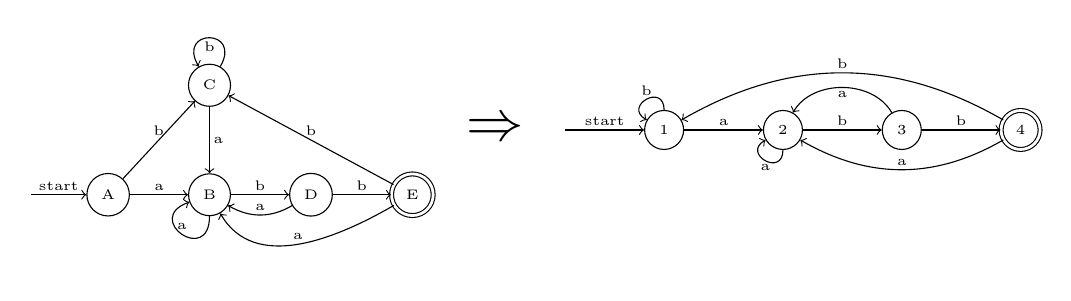
\begin{tikzpicture}
  % DFA
  \node[text width=-3em](DFAstart){\tiny};
  \node[circle, draw=black, right=2em of DFAstart](DFAA){\tiny A};
  \node[circle, draw=black, right=2.1em of DFAA](DFAB){\tiny B};
  \node[circle, draw=black, above=2.4em of DFAB](DFAC){\tiny C};
  \node[circle, draw=black, right=2.1em of DFAB](DFAD){\tiny D};
  \node[circle, double, double distance=1pt, draw=black, right=2.1em of DFAD](DFAE){\tiny E};

  \path[->]
  (DFAstart) edge node[above=-2pt]{\tiny start} (DFAA)
  (DFAA) edge node[above=-2pt]{\tiny a} (DFAB)
  (DFAA) edge node[above=-2pt]{\tiny b} (DFAC)
  (DFAB) edge[out=270, in=200, min distance=1.8em] node[above=-2pt]{\tiny a} (DFAB)
  (DFAB) edge node[above=-2pt]{\tiny b} (DFAD)
  (DFAC) edge node[right=-2pt]{\tiny a} (DFAB)
  (DFAC) edge[out=60, in=120, min distance=1.6em] node[below=-2pt]{\tiny b} (DFAC)
  (DFAD) edge[out=210, in=330] node[above=-2pt]{\tiny a} (DFAB)
  (DFAD) edge node[above=-2pt]{\tiny b} (DFAE)
  (DFAE) edge[out=210, in=300] node[above=-2pt]{\tiny a} (DFAB)
  (DFAE) edge node[above=-2pt]{\tiny b} (DFAC);

  % transition
  \node[above right=1.5em of DFAE](arrow){\huge $\Rightarrow$};

  % min
  \node[text width=-3em, right=1em of arrow](start){\tiny};
  \node[circle, draw=black, right=of start](A){\tiny 1};
  \node[circle, draw=black, right=of A](B){\tiny 2};
  \node[circle, draw=black, right=of B](C){\tiny 3};
  \node[circle, double, double distance=1pt, draw=black, right=of C](D){\tiny 4};

  \path[->]
  (start) edge node[above=-2pt]{\tiny start} (A)
  (A) edge[out=90, in=150, min distance=1em] node[above=-2pt]{\tiny b} (A)
  (A) edge node[above=-2pt]{\tiny a} (B)
  (B) edge[out=270, in=210, min distance=1em] node[below=-2pt]{\tiny a} (B)
  (B) edge node[above=-2pt]{\tiny b} (C)
  (C) edge[out=120, in=60] node[below=-2pt]{\tiny a} (B)
  (C) edge node[above=-2pt]{\tiny b} (D)
  (D) edge[out=150, in=30] node[above=-2pt]{\tiny b} (A)
  (D) edge[out=210, in=330] node[above=-2pt]{\tiny a} (B);
\end{tikzpicture}

\end{document}
